\section{Probability distributions}

\subsection{Normal}

By contrast with substantial majority of books, the univariate normal distribution
can be derived form the multivariate normal distribution.
In this section we show how to obtain the univariate normal from the bivariate.

\begin{marginfigure}
  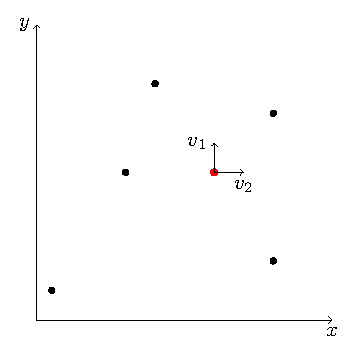
\includegraphics[width=\linewidth]{figures/04_normal.pdf}
  \caption{Black dots represent the gas molecules.
  The red dot stands for the one we catch.
  Its speed along the horizontal axis is $v_1$, i.e., the first component of
  the velocity vector, and its speed along the vertical axis is $v_2$.}
\end{marginfigure}

The original idea belongs to J.C. Maxwell who was wondering
what distribution the velocity of gas molecules follow.
The similar question was also bothering J.H.W. Herschel who was an astronomer
and was dealing with measurement errors in astronomical data.
Here we provide a proof of the theorem known today as Herschel-Maxwell's.

Assume there are gas molecules moving chaotically on a plane
and we can measure the velocity vector of one of them.
We will denote this vector as $V = \begin{pmatrix} X \\ Y \end{pmatrix}$
where $X$ and $Y$ stand for the horizontal and vertical components respectively.
Assume additionally that
\begin{enumerate}
  \item The joint distribution finction $f(x,y)$ does not depend on
  the vector $(X,Y)^T$ direction but depends on its length only;
  \item The orthogonal components of the velocity vector are independent;
  \item And we measure the velocity in such a way that $\Var(X) = 1$.
\end{enumerate}

\marginnote{
It is more common to introduce a standard normal distribution in terms of its PDF
\begin{definition}
A continuous random variable $\xi$ has a standard normal distribution
if its PMF is given by
\[
f_{\xi} (x) = \frac{1}{\sqrt{2\pi}}\exp\left(-\frac{x^2}{2}\right).
\]
\end{definition}
After that multivariate normal is defined.

\begin{definition}
Let $\xi_i \stackrel{iid}{\sim} \mathcal{N}(0, 1)$ then $\xi \sim \mathcal{N}(\vec{0}, I)$
where $\xi = \begin{pmatrix} \xi_1 \\ \vdots \\ \xi_n \end{pmatrix}$,
$I$ is $n \times n$ identity matrix, and its PMF is
\[
f_{\xi} (x_1, \ldots, x_n) = \frac{1}{(\sqrt{2\pi})^n}\exp\left(-\frac{x_1^2+\ldots+x_n^2}{2}\right).
\]
\end{definition}
And finally, location-scale transformations are applied.
}

\begin{theorem}
Assumptions (1), (2) and (3) are satisfied if and only if
$X \sim \mathcal{N}(0, 1)$, $Y \sim \mathcal{N}(0, 1)$
and $X$, $Y$ are independent.
\end{theorem}

\begin{proof}
First of all, consider a vector $V' = \begin{pmatrix} -Y \\ X \end{pmatrix}$, i.e.,
the original vector $V$ rotated $90^{\circ}$ counterclock-wise.
By the assumption (1), this operation did not change the distribution of $V$.
Hence, $V' \sim V$ which implies $-Y \sim X$ and $X \sim Y$.
It follows that
\[
\begin{cases}
\E(-Y) = \E(X) \\
\E(X) = \E(Y)
\end{cases}
\]
which holds for $\E(X) = \E(Y) = 0$ only.
One may notice that $\E(X)$ may not exist at all,
but we derive later the exact distribution of $X$.

Likewise, $\Var(X) = \Var(Y)$ and it follows from the assumption (3)
that $\Var(X) = \Var(Y) = 1$.

Next, we introduce the angle between $V$ and the horizontal axis $U$ and
the length of the velocity vector $R = \sqrt{X^2 + Y^2}$.
Obviously, $X = R \cos U$ and $Y = R \sin U$.
Note that since the joint distribution of $X$ and $Y$ depends only on
the length of vector $V$ the distribution function of $U$ can only be constant,
thus variable $U$ is uniform on the interval $(0, 2\pi)$.

Applying assumption (1) again, we conclude that the joint distribution function
can be written as a function of the length of the velocity vector, or equivalently
of the length squared:
\[
f(x,y) = h(x^2 + y^2).
\]
By the assumption (2), orthogonal components of $V$ are independent.
Hence, the joint PMF can be decomposed to the product of marginal ones:
\[
f(x,y) = f(x)f(y) = g(x^2)g(y^2)
\]
where the latter equality was written for convenience.
Putting everything together, we obtain
\[
h(x^2 + y^2) = g(x^2)g(y^2).
\]
Next, we take the derivative of both sides with respect to $y^2$ and
then substitute $y^2 = 0$ to get a constant $k$:
\begin{align*}
h'(x^2 + y^2) &= g(x^2)g'(y^2) \\
h'(x^2) &= g(x^2)g'(0) \\
h'(x^2) &= k \cdot g(x^2)
\end{align*}

\marginnote{
In order to obtain $k$ we computed
\begin{align*}
\E(X^2) &= \int_{-\infty}^{\infty} x^2 \sqrt{c} e^{kx^2} dx \\
&= \left. x \cdot \sqrt{c} e^{kx^2} \cdot \frac{k}{2} \right|_{-\infty}^{\infty} - \int_{-\infty}^{\infty} \sqrt{c} e^{kx^2} \cdot \frac{1}{2k} dx \\
&= - \frac{1}{2k} \int_{-\infty}^{\infty} \sqrt{c} e^{kx^2} \\
&= - \frac{1}{2k} \cdot 1 \\
&= 1.
\end{align*}
}

Solving the differential equation, we obtain
\[
h(x^2) = c e^{kx^2}, \quad c \in \mathbb{R}.
\]
So the joint PMF can be written as follows:
\[
f(x,y) = h(x^2 + y^2) = c e^{k(x^2+y^2)}
\]
and due to independece of $X$ and $Y$ the PMF of $X$ is
\[
f(x) = \sqrt{c} e^{kx^2}.
\]

\marginnote{
In order to obtain $c$ we computed:
\begin{align*}
\int_{-\infty}^{\infty} \int_{-\infty}^{\infty} e^{-\frac{x^2 + y^2}{2}} dx dy &= \int_{0}^{2\pi} \int_{0}^{\infty} e^{-\frac{r^2}{2}}r dr d\theta \\
&= \int_{0}^{2\pi} \left(\int_{0}^{\infty} e^{-u} du \right) d\theta \\
&= \int_{0}^{2\pi} 1 d\theta \\
&= 2 \pi.
\end{align*}
}

In order to find the constant $k$, we need to solve $\E(X^2) = 1$.
Computing the integral we obtain $k=-\frac{1}{2}$.

Finally, we need to normalize $f(x, y) = c e^{-\frac{x^2 + y^2}{2}}$ so as to
obtain $c$. Again, computing another integral,
we conclude that $c=(2\pi)^{-1}$ which finishes the proof.

Without assumption (3) variables $X$ and $Y$ are normal $\mathcal{N}(0, \sigma^2)$.
\end{proof}

Notice, that any other $\mathcal{N}(\mu, \sigma^2)$ can be obtained by applying
location-scale transformations.

The theorem can be generalized to the $n$-dimensional case.
\begin{theorem}\label{th:mvn}
The vector $z = \begin{pmatrix} z_1 \\ \vdots \\ z_n \end{pmatrix}$
follows the standard multivariate normal distribution and its components
are independent if and only if
\begin{enumerate}
  \item the function $f(z)$ depends on $\lVert z \rVert$ only,
  \item the projections of vector $z$ onto the orthogonal subspaces $A$ and $B$
  in $\mathbb{R}^n$ are independent.
\end{enumerate}
\end{theorem}


\subsection{Chi-squared}

\marginnote{
\begin{definition}\label{def:chi_traditional}
Let $z_i \stackrel{iid}{\sim} \mathcal{N}(0,1)$.
Then $Q$ follows the chi-squared distribution with $k$ degrees of freedom
if it can be written as
\[
Q = z_1^2 + z_2^2 + \ldots + z_k^2.
\]
\end{definition}

This definition is a particular case of the geometric one.
Consider projecting a vector $z = (z_1, z_2, \ldots, z_n)$ form $\mathbb{R}^n$
onto the~$k$-dimensional subspace $S$ of vectors which first $k$ coordinates
are arbitrary and all the rest are zeros. As a result we would get
\[
\hat z = (z_1, z_2, \ldots, z_k, 0, \ldots, 0).
\]
Squaring the length of the projection, we obtain
\[
Q = \lVert \hat z \rVert = z_1^2 + z_2^2 + \ldots + z_k^2.
\]
}

\begin{definition}\label{th:chi}
Consider a random vector $z \in \mathbb{R}^n$ which components are independent
and follow standard normal distribution, $z_i \sim \mathcal{N}(0,1)$.
Consider also a $k$-dimensional subspace $L$ in $\mathbb{R}^n$.
Let the projection of vector $z$ onto the subspace $L$ be $\hat z$ and
its length squared $Q$
\[
Q = \lVert \hat z \rVert^2 = \langle \hat z, \hat z \rangle = \hat z^T \hat z
\]
Then $Q$ follows the chi-squared distribution with $k$ degrees of freedom.
\end{definition}

\begin{theorem}
The definitions~\ref{def:chi_traditional} and \ref{th:chi} are equivalent.
\end{theorem}

\begin{proof}
First, it can be shown that the~projected vector $\hat z$ is the~original vector $z$
multiplied by the~projection matrix $H = X(X^T X)^{-1}X^T$ where the columns of $X$
are fixed linearly independent vectors $x_1, \ldots, x_k$ in $L$
or equivalently $\col X = \Lin(x_1, \ldots, x_k)$.
This matrix is  also often referred to as `hat-matrix'.
Then the statement in~the~theorem can be rewritten as follows:
\[
\hat z^T \hat z = (Hz)^T Hz = z^T H^T H z = z^T H^2 z = z^T H z,
\]
applying the idempotence property in the last step.

Another nice property of~the~hat-mattix is symmetry.
Thus, it can be decomposed as
\[
H = P D P^T,
\]
where we choose the vectors of matrix $P$ to be unit and orthogonal,
and $D = \diag{(\lambda_1, \ldots, \lambda_n)}$ where $\lambda_i$ is an eigenvalue of $H$.

\begin{marginfigure}
  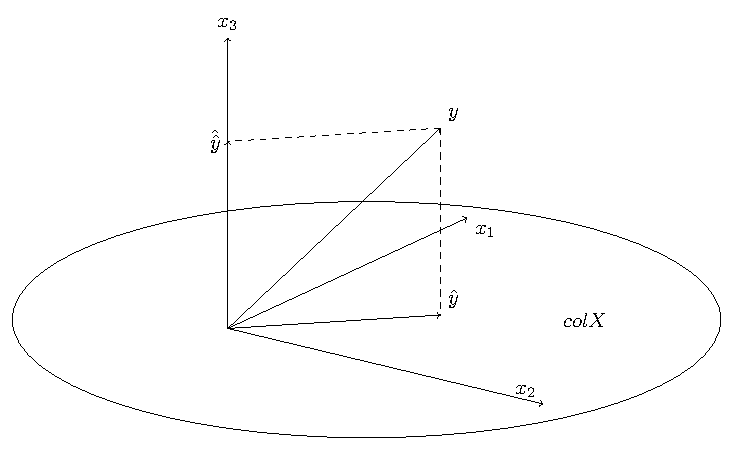
\includegraphics[width=\linewidth]{figures/04_chi_squared_example.pdf}
  \caption{Consider a $3$-dimensional example, $\col X = \Lin(x_1, x_2)$ and $col^{\perp}X = \Lin(x_3)$.
  $H x_1 = x_1$ and $H x_2 = x_2$ since they are in $\col X$. However, $H x_3 = 0$ as $x_3 \perp \col X$.
  Projecting an arbitrary vector onto $\col X$ yileds $Hy = \hat y \in \Lin(x_1, x_2)$
  while projecting onto $\col^{\perp}X$ results in $(I-H)y = \hat{\hat y} \in \Lin(x_3)$.}
\end{marginfigure}

Since $H^2 = H$ the eigenvalues are either $0$ or $1$.
Recall that $H$ projects a vector onto $\col X$.
Then for any $x_i$, $i = 1, \ldots, k$, $H x_i = x_i \cdot 1$ since
any $x_i$ is already in $\col X$. This implies that $\lambda_1 = \ldots = \lambda_k = 1$.
There are also $n-k$ vectors in the subspace orthogonal to $\col X$.
So for any $x_i$, $i= k+1, \ldots, n$, the orthogonal projection yields zero.
We conclude that $\lambda_{k+1} = \ldots = \lambda_n = 0$.

Rewritting the theorem statement further, we obtain
\[
z^T H z = z^T P D P^T z = (P^T z)^T D (P^T z) = \tilde z^T D \tilde z = \tilde z_1^2 + \ldots + \tilde z_k^2.
\]
Now we explore $\tilde z$ given $z \sim \mathcal{N}(0, I)$:
\begin{align*}
&\tilde z = P^T z \\
&\E(\tilde z) = \E(P^T z) = P^T \E(z) = 0 \\
&\Var(\tilde z) = \Var(P^T z) = P^T \Var(z) (P^T)^T = P^T P = I
\end{align*}
So we conclude that $\tilde z_1^2 + \ldots + \tilde z_k^2 \sim \chi^2_k$.

\end{proof}


\subsection{Student's}

\marginnote{
A continuous random variable $T$ has Student's distribution with $k$ degrees
of freedom if it can be expressed as
\[
T = \frac{Z}{\gamma_k/\sqrt{k}},
\]
where $Z \sim \mathcal{N}(0,1)$, $\gamma_k \sim \chi^2_{k}$ and
$Z$, $\gamma_k$ are independent.
}

\begin{definition}
Let  $z = \begin{pmatrix} z_1 \\ \vdots \\ z_n \end{pmatrix}$
where $z_i \sim \mathcal{N}(0, \sigma^2), i=1, \ldots, n$ and are independent.
Let $L_1$ be 1-dimensional subspace in $\mathbb{R}^{n}$,
generated by unit-length vector $a$, $L_1 = \Lin(a)$.
Let $L_2$ be a subspace orthogonal to $L_1$.
Let $T$ be a scaled ratio of lengths:
\[
T = \frac{\langle a, z \rangle}{\lVert H_2 z \rVert / \sqrt{\dim L_2}}
\]
where $\langle a, x \rangle$ is the length of the projection of vector $z$ onto
1-dimensional subspace $L_1$ multiplied by plus or minus one,
$\lVert H_2 z \rVert$ — the length of the projection of vector $z$ onto $L_2$,
Then $T$ follows Student's distribution with $\dim L_2$ degrees of freedom.
\end{definition}

% Let us choose two orthogonal subspaces: one-dimensional $L_1$ and $k$-dimensional $L_2$.

Previously we showed that, the squared length of projection follows
the chi-squared distribution with the degrees of freedom equal to the dimension
onto which the vector was projected. Thus, $\langle a, z \rangle^2 = \lVert H_1 z \rVert^2 \sim \chi^2_1$
and $\lVert H_2 z \rVert^2 \sim \chi^2_{k}$.
Now we can express $T^2$ as a ratio of the per-dimension lengths squared:
\[
T^2 = \frac{\lVert H_1 z \rVert^2}{\lVert H_2 z \rVert^2 / \dim L_2}
\]
Taking the square root of both sides, we obtain:
\[
T = \frac{\langle a, z \rangle}{\lVert H_2 z \rVert / \sqrt{\dim L_2}} = \tg \varphi \sqrt{\dim L_2}
\]
The latter equality can be illustarted with a $3$-dimensional example (see Figure~\ref{fig:f_dist}).





\subsection{t-test}

In a simple linear regression model
\[
y = \beta_1 \mathbf{1} + \beta_2 x + \varepsilon
\]
the adjusted t-value $\frac{t}{\sqrt{n-2}}$ when $H_0: \beta_2 = 0$ is tested
can be expressed in terms of the angle between $y$ and $\hat y$ $\varphi$ and
is equal to $\ctg \varphi$.

Recall that the t-statistic is defined in the following way:
\[
t = \frac{\hat \beta - \beta}{se\left(\hat\beta\right)}
\]
Adjusting this formula for the null hypothesis $H_0: \beta_2 = 0$, we obtain
\begin{equation}\label{eq:tstat}
t = \frac{\hat \beta_2}{se\left(\hat\beta_2\right)}
\end{equation}
Then, we need to express $se\left(\hat\beta_2\right)$ in terms of vectors which can be
plotted. From standard OLS procedure it follows that
\begin{equation}\label{eq:varbeta2}
\Var(\hat \beta_2) = \frac{\sigma^2}{\sum\limits_{i=1}^n (x_i - \bar x)^2}
\end{equation}
Since actual $\sigma$ is unknown the estimator will be used instead:
\begin{equation}\label{eq:sigmaest}
\hat \sigma^2 = \frac{RSS}{n-2}
\end{equation}
Substituting \eqref{eq:varbeta2} and \eqref{eq:sigmaest} into \eqref{eq:tstat}
divided by $\sqrt{n-2}$, we obtain
\begin{align*}
\frac{t}{\sqrt{n-2}} &=
\frac{\hat \beta_2}{\sqrt{n-2}se\left(\hat\beta_2\right)} =
\frac{\hat \beta_2}{\sqrt{n-2}\frac{\hat \sigma}{\sqrt{\sum\limits_{i=1}^n (x_i - \bar x)^2}}} \\
&= \frac{\hat \beta_2 \sqrt{\sum\limits_{i=1}^n (x_i - \bar x)^2}}{\sqrt{n-2}\frac{\sqrt{\sum\limits_{i=1}^n (y_i - \hat y_i)^2}}{\sqrt{n-2}}} =
\frac{\hat \beta_2 \lVert x^c \rVert}{\sqrt{RSS}}
\end{align*}
where $ \lVert x^c \rVert = \sqrt{\sum_{i=1}^n (x_i - \bar x)^2}$ is the length of the
centred vector $x$.

Now the result can be demonstrated visually.
Again we will project $x$ and $y$ vectors onto the $\Lin^{\perp}(\mathbf{1})$ so as to
get their centred versions $x^c$ and $y^c$.
Then, we perform regression of $y$ onto $\Lin(x, \mathbf{1})$ which results in $\hat y$.
Following that, we project $\hat y = \hat \beta_1 \mathbf{1} + \hat \beta_2 x$ onto $\Lin^{\perp}(\mathbf{1})$
which yields $\hat \beta_2 x^c$.
After all, we translate $\sqrt{RSS}$ onto $\Lin^{\perp}(\mathbf{1})$.
These steps are demonstrated in Figure~\ref{fig:ttest_3d}.

Looking at Figure~\ref{fig:ttest_lin} which depicts the $\Lin^{\perp}(\mathbf{1})$,
we derive
\[
\ctg \varphi = \frac{\hat \beta_2 \lVert x^c \rVert}{\sqrt{RSS}} = \frac{t}{\sqrt{n-2}}
\]

\begin{figure}[ht!]
\begin{center}
\subfigure[]{
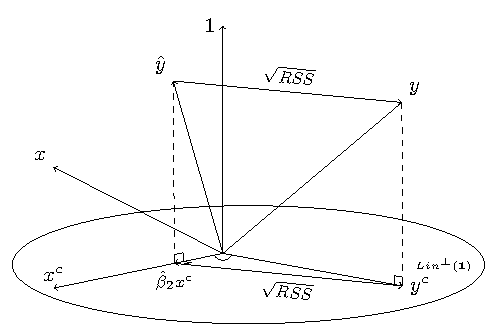
\includegraphics[width=0.45\linewidth]{figures/04_ttest.pdf}
\label{fig:ttest_3d}}
%\hspace{4ex}
\subfigure[]{
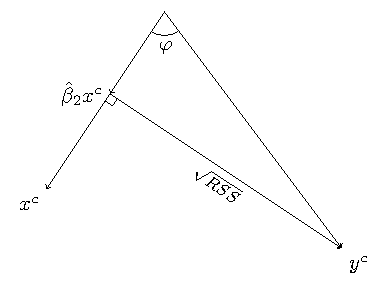
\includegraphics[width=0.45\linewidth]{figures/04_ttest_lin.pdf}
\label{fig:ttest_lin}}
\caption{\subref{fig:pcorr_t_x}: Regression of $y$ onto $\Lin(x, \mathbf{1})$ and appropriate projections;
\subref{fig:pcorr_t_y}: $\Lin^{\perp}(\mathbf{1})$.}
\end{center}
\end{figure}


\subsection{F-distribution}

\marginnote{
Generally, the following definition is given.
\begin{definition}
Let $\gamma_1 \sim \chi^2_{k_1}$, $\gamma_2 \sim \chi^2_{k_2}$,
$\gamma_1$, $\gamma_2$ independent.
Then
\[
\frac{\gamma_1/k_1}{\gamma_2/k_2} \sim F_{k_1, k_2}.
\]
\end{definition}
}

\begin{definition}\label{def:f}
Let $z = \begin{pmatrix} z_1 \\ \vdots \\ z_n \end{pmatrix}$
where $z_i \sim \mathcal{N}(0, \sigma^2)$ and are independent.
Let $L_1$, $L_2$ be orthogonal subspaces in $\mathbb{R}^n$.
then
\[
F = \frac{\lVert H_1 z \rVert^2 / \dim L_1}{\lVert H_2 z \rVert^2 / \dim L_2} \sim F_{\dim L_1, \dim L_2},
\]
where $\lVert H_1 z \rVert^2$, $\lVert H_2 z \rVert^2$ are the squared lengths
of $z$ projected onto $L_1$ and $L_2$ respectively.
\end{definition}

Recall that by Theorem~\ref{th:mvn} the projections of a standard noraml vector
onto orthogonal subspaces are independent.
Thus, in terms of the Definition~\ref{def:f} $H_1 z$ and $H_2 z$ are independent.
Next, from the Definition~\ref{th:chi} where we defined the chi-squared distribution
it follows that the squared lengths of these projections follow
the chi-squared distribution with the number of degrees of freedom
equal to the dimension of the subspace onto which the vector was projected.
In other words, $\lVert H_1 z \rVert^2 \sim \chi^2_{\dim L_1}$,
$\lVert H_2 z \rVert^2 \sim \chi^2_{\dim L_2}$.

\begin{marginfigure}
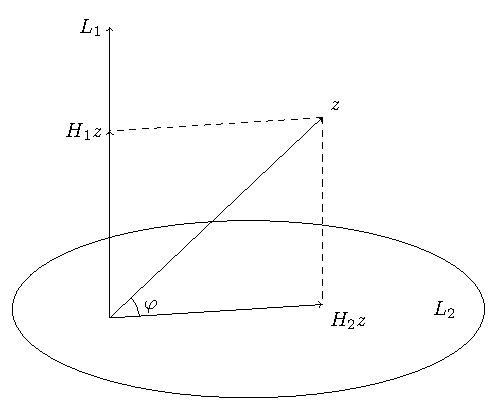
\includegraphics[scale=0.7]{figures/04_f_dist_example.pdf}
\caption{F-distribution as the ratio of the projection lengths squared
adjusted to the dimensions of the subspaces.}
\label{fig:f_dist}
\end{marginfigure}

Taking the ratio of these length squared, we get the interpretaion
of the angle between the original vector $z$ and its projection onto $L_1$:
\[
\tg^2 \varphi = \frac{\lVert H_1 z \rVert^2}{\lVert H_2 z \rVert^2}.
\]
Adjusting this ratio to the degrees of freedom, we get the desired definition.


\subsection{F-test}

The significance of several coefficients at once can be tested with the F-test.
The F-statistic has the following form
\[
F = \frac{(RSS_{R} - RSS_{UR})/q}{RSS_{UR}/(n-k_{UR})}
\]
where indices $R$ and $UR$ stand for the restricted and unrestricted models
respectively, $n$ — number of observations, $k$ — number of regressors,
$q$ — number of equtions used in the null hypothesis.

\begin{marginfigure}
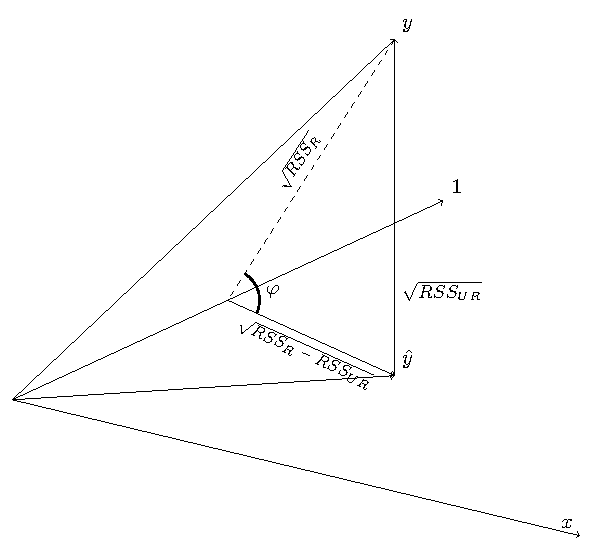
\includegraphics[scale=0.55]{figures/04_ftest.pdf}
\caption{F-statistic is proportional to the cotangent squared of $\varphi$,
where $a$ stands for $\sqrt{RSS_{UR}}$, $b$ — $\sqrt{RSS_{R} -RSS_{UR}}$,
$c$ — $\sqrt{RSS_{R}}$.}
\label{fig:ftest}
\end{marginfigure}

Due to plotting limitations, we consider the unrestricted model to be
\[
y = \beta_1 \mathbf{1}+ \beta_2 x + u
\]
and the restricted model to be
\[
y = \alpha_1 \mathbf{1} + v
\]
Note that there was a choice in the restricted models.


We perform both regressions in order to get the ressiduals and plot them
in Figure~\ref{fig:ftest}.
Adjusted to the degrees of freedom, the ratio can be expressed in terms of the
angle between two vectors, $\varphi$, as demonstrated in Figure~\ref{fig:ftest}
\[
F = \frac{(RSS_{R} - RSS_{UR})/q}{RSS_{UR}/(n-k_{UR})} =
\ctg^2 \varphi \cdot \frac{n - k_{UR}}{q}
\]
